%%%%%%%%%%%%%%%%%%%%%%%%%%%%%%%%%%%%%%%%%
% Beamer Presentation
% LaTeX Template
% Version 1.0 (10/11/12)
%
% This template has been downloaded from:
% http://www.LaTeXTemplates.com
%
% License:
% CC BY-NC-SA 3.0 (http://creativecommons.org/licenses/by-nc-sa/3.0/)
%
%%%%%%%%%%%%%%%%%%%%%%%%%%%%%%%%%%%%%%%%%

%----------------------------------------------------------------------------------------
%	PACKAGES AND THEMES
%----------------------------------------------------------------------------------------

\documentclass{beamer}

\mode<presentation> {

% The Beamer class comes with a number of default slide themes
% which change the colors and layouts of slides. Below this is a list
% of all the themes, uncomment each in turn to see what they look like.

%\usetheme{default}
%\usetheme{AnnArbor}
%\usetheme{Antibes}
%\usetheme{Bergen}
%\usetheme{Berkeley}
%\usetheme{Berlin}
%\usetheme{Boadilla}
%\usetheme{CambridgeUS}
%\usetheme{Copenhagen}
%\usetheme{Darmstadt}
%\usetheme{Dresden}
%\usetheme{Frankfurt}
%\usetheme{Goettingen}
%\usetheme{Hannover}
%\usetheme{Ilmenau}
%\usetheme{JuanLesPins}
\usetheme{Luebeck}
%\usetheme{Madrid}
%\usetheme{Malmoe}
%\usetheme{Marburg}
%\usetheme{Montpellier}
%\usetheme{PaloAlto}
%\usetheme{Pittsburgh}
%\usetheme{Rochester}
%\usetheme{Singapore}
%\usetheme{Szeged}
%\usetheme{Warsaw}

% As well as themes, the Beamer class has a number of color themes
% for any slide theme. Uncomment each of these in turn to see how it
% changes the colors of your current slide theme.

%\usecolortheme{albatross}
%\usecolortheme{beaver}
%\usecolortheme{beetle}
%\usecolortheme{crane}
%\usecolortheme{dolphin}
%\usecolortheme{dove}
%\usecolortheme{fly}
%\usecolortheme{lily}
%\usecolortheme{orchid}
%\usecolortheme{rose}
%\usecolortheme{seagull}
%\usecolortheme{seahorse}
%\usecolortheme{whale}
%\usecolortheme{wolverine}

%\setbeamertemplate{footline} % To remove the footer line in all slides uncomment this line
%\setbeamertemplate{footline}[page number] % To replace the footer line in all slides with a simple slide count uncomment this line

%\setbeamertemplate{navigation symbols}{} % To remove the navigation symbols from the bottom of all slides uncomment this line
}

\usepackage{graphicx} % Allows including images
\usepackage{booktabs} % Allows the use of \toprule, \midrule and \bottomrule in tables
%----------------------------------------------------------------------------------------
%	TITLE PAGE
%----------------------------------------------------------------------------------------

\title[Email Spoofing]{Introduction to Email Spoofing and Prevention} % The short title appears at the bottom of every slide, the full title is only on the title page

\author{Sumit Agrawal
        \and
        Piyush Lahoti
        } % Your name
\institute[IITI] % Your institution as it will appear on the bottom of every slide, may be shorthand to save space
{
Indian Institute of Technology Indore \\ % Your institution for the title page
\medskip
\textit{sumit4iit@gmail.com\\ piyush@iiti.ac.in} % Your email address
}
\date{\today} % Date, can be changed to a custom date

\begin{document}

\begin{frame}
\titlepage % Print the title page as the first slide
\end{frame}

\begin{frame}
\frametitle{Overview} % Table of contents slide, comment this block out to remove it
\tableofcontents % Throughout your presentation, if you choose to use \section{} and \subsection{} commands, these will automatically be printed on this slide as an overview of your presentation
\end{frame}

%\begin{frame}
%  \frametitle{Figures}
%  \listoffigures
%\end{frame}

%----------------------------------------------------------------------------------------
%	PRESENTATION SLIDES
%----------------------------------------------------------------------------------------
% Slide 1- Introdction
%------------------------------------------------
\section{Email Protocols} % Sections can be created in order to organize your presentation into discrete blocks, all sections and subsections are automatically printed in the table of contents as an overview of the talk
%------------------------------------------------


\begin{frame}
\frametitle{Email Protocols}

Interaction between email servers is governed by email protocols.
\begin{itemize}
  \item Simple Mail Transfer Protocol
  \item Internet Message Access Protocol
  \item Post Office Protocol
\end{itemize}

\end{frame}

%------------------------------------------------
\subsection{Post Office Protocol: POP} % A subsection can be created just before a set of slides with a common theme to further break down your presentation into chunks
\begin{frame}
  \frametitle{Post Office Protocol}
  \begin{itemize}
    \item Oldest Protocol: (Recent- POP3[1984])
    \item Clients using POP generally connect, retrive all messages and store them on the user's PC as new    message, delete from the server and then disconnect. 
    \item POP3S
    \item No notion of folders.
  \end{itemize}
\end{frame}
%------------------------------------------------
\begin{frame}
  \frametitle{Post Office Protocol}
  \framesubtitle{Working}
  \begin{figure}[h]
    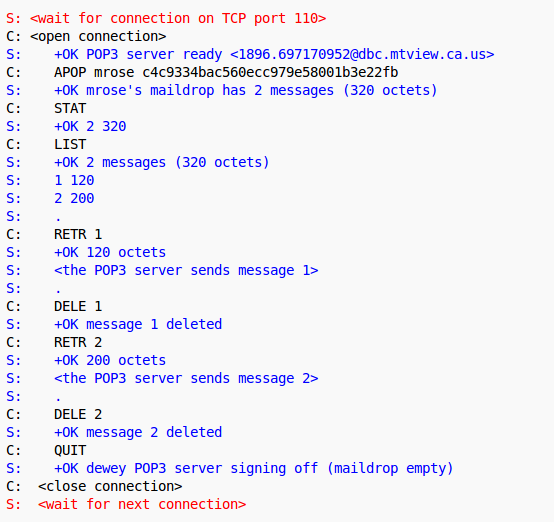
\includegraphics[scale = 0.35]{pop3.png}
    \caption{Demonstration of POP.}
    \centering
  \end{figure}
\end{frame}
%------------------------------------------------
\subsection{Internet Message Access Protocol}
\begin{frame}
  \frametitle{Internet Message Access Protocol}
  \begin{itemize}
    \item Defaults to leaving message on email server. Simply downloads a local copy.
    \item Has notion of folders and hence mailbox is more organized.
    \item Can perform complex queries. Has ability to retrive partial messages. Allows labeling of emails e.g. read, unread.
    \item Designed to treat remote mailboxes as if they were local.
    \item In contrast to POP multiple clients can connect to server on same mailbox.
  \end{itemize}
  
\end{frame}
%------------------------------------------------
\begin{frame}
  \frametitle{Internet Message Access Protocol}
  \framesubtitle{Working}
  \begin{figure}[h]
    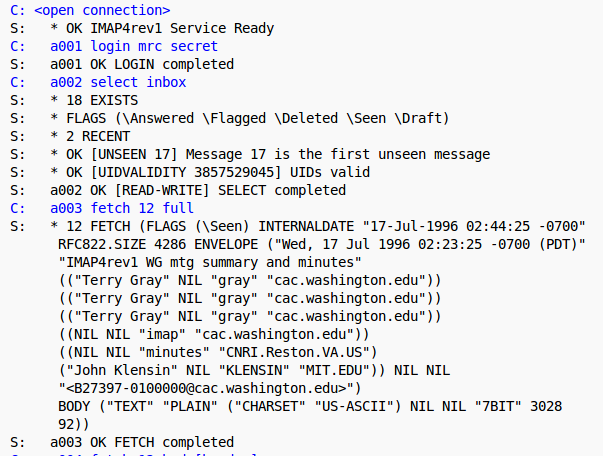
\includegraphics[scale = 0.35]{imap1.png}
    \caption{Demonstration of IMAP.}
    \centering
  \end{figure}
\end{frame}
%------------------------------------------------
\begin{frame}
  \frametitle{Internet Message Access Protocol}
  \framesubtitle{Working}
  \begin{figure}[h]
    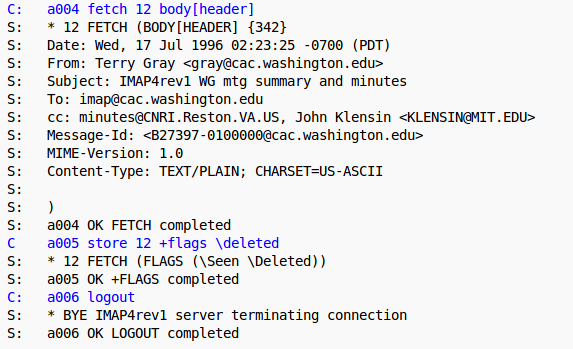
\includegraphics[scale = 0.35]{imap2.png}
    \caption{Demonstration of IMAP.}
    \centering
  \end{figure}
\end{frame}
%------------------------------------------------
\subsection{Simple Mail Transfer Protocol}
\begin{frame}
  \frametitle{Simple Mail Transfer Protocol}
  \begin{itemize}
    \item We use IMAP and POP to \emph{receive emails}. We \emph{send} emails using SMTP
    \item Email is submitted by client using MUA \emph{(Mail User Agent)} which is delivered to MTA \emph{(Mail Transfer Agent)}.
    \item MTA performs DNS lookup to lookup MX \emph{(Mail eXchanger)} records. MTA next connects to MX server as SMTP client.
    \item Once target MX accepts the message it hands it over to MDA \emph{(Mail Delivery Agent)}. MDA further saves message in relevant message format.
    \item Further end user clients connect to server using POP or IMAP to access emails.
  \end{itemize}
\end{frame}
%------------------------------------------------
\begin{frame}
  \frametitle{Simple Mail Transfer Protocol}
  \framesubtitle{Working}
  \begin{figure}[h]
    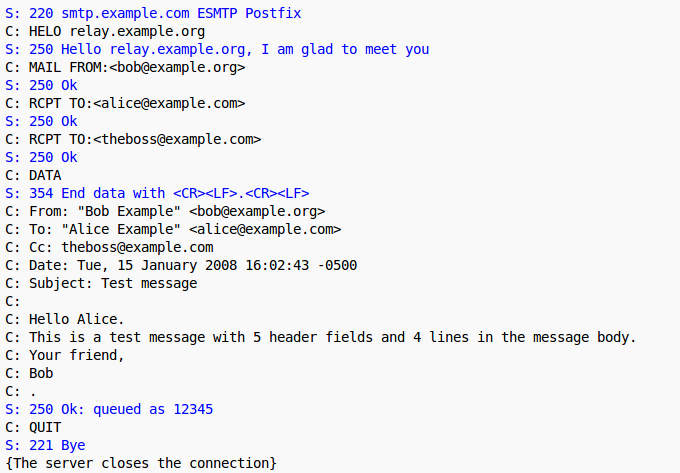
\includegraphics[scale = 0.35]{SMTP.png}
    \caption{Demonstration of SMTP.}
    \centering
  \end{figure}
\end{frame}
%------------------------------------------------
\section{Issues}
\subsection{Open Mail Relay}
\begin{frame}
  \frametitle{Open Mail Relay}
  \begin{itemize}
    \item An \emph{open mail relay} is an SMTP server configured such that it allows any one on the Internet to send emails through it. 
    \item Spammers would sent one email to openrelay and include a large bcc list, then the open relay would spam the entire list.
    \item Hashbusters
    \item Closing relays: Mailboxes should not accept and forward arbitrary e-mails from non-local ip addresses to non-local mailboxes by an unauthenticated or unauthorized user.
    
  \end{itemize}
\end{frame}
%------------------------------------------------
\section{Defense}
\subsection{SPF}
\begin{frame}
  \frametitle{Sender Policy Framework}
  \begin{itemize}
    \item SPF allows administrators to specify which hosts are allowed to send mail from a given domain by creating a specific spf record (can be specified using TXT as well).
    \item example.net TXT "v=spf1 mx a:p.example.net include:aspmx.googlemail.com -all"
  \end{itemize}
\end{frame}
%------------------------------------------------
\begin{frame}
  \frametitle{Sender Policy Framework: Contd.}
  \begin{itemize}
    \item If domain publishes a SPF record, spammers and phishers are less likely to forge e-mails from that domain. 
    \item Issues in case of forwarding:
    \item Forwarder does not rewrite a return path.
    \item The next hop does not white list the forwarder
  \end{itemize}
\end{frame}
%------------------------------------------------
\subsection{DKIM}
\begin{frame}
  \frametitle{Domainkeys Identified Mail}
  \begin{itemize}
    \item DKIM is a way to associate domain name with email. This association is set up by means of digital signature which can be verified by recepients.
    \item Similar to PK Infrastructure.
    \item Singer claims responsibility by adding a DKIM signature field to message's header. The verifier recovers singer's public key using dns lookup and verifies that signature matches message's contents. 
  \end{itemize}
\end{frame}
%------------------------------------------------
\begin{frame}
  \frametitle{Domainkeys Identified Mail: Working}
  \begin{figure}[h]
    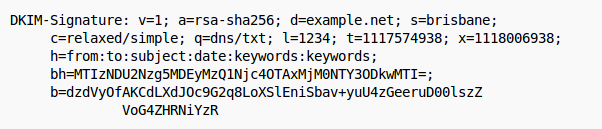
\includegraphics[scale = 0.35]{dkim.png}
    \caption{Demonstration of SMTP.}
    \centering
  \end{figure}
  \begin{itemize}
    \item b: body + headers [signature]
    \item bh: body [Hash]
    \item d: signing domain
    \item s: selector
%      
  \end{itemize}

\end{frame}
%------------------------------------------------
\begin{frame}
  \frametitle{Domainkeys Identified Mail: Working}
  \begin{itemize}
%    \item verifier queries the TXT records brisbane._domainkey.example.net.
    \item v: version
    \item a: signing algorithm 
    \item c: canonicalization algorithm
    \item q: default query method
    \item l: length of the canonicalized part of the body that has been signed.
    \item t: signature time
    \item x: expire time
    \item h: list of signed header fields.
  \end{itemize}
\end{frame}


\end{document} 
